\documentclass{article}
\usepackage[UTF8, scheme = plain]{ctex} % {ctex} 包用于处理中文支持;[UTF8] 是一种广泛使用的字符编码,支持多种语言的字符,包括中文;[scheme = plain]:设置 ctex 包的样式方案为 plain,plain 方案提供了最基础的中文支持,不包含额外的格式设置或字体调整,适用于那些需要在基本 LaTeX 文档中添加中文支持的场合
\usepackage{amsmath} % 提供额外的环境(如 align, equation, split, multline 等),支持多行公式的对齐和子公式的编号等高级功能
\usepackage{amssymb} % 扩展的数学符号集,通常与 amsmath 宏包一起使用
\usepackage{amsthm} % 用于排版数学定理、定义、证明等结构
\usepackage{graphicx} % 支持在 LaTeX 文档中插入图像(JPEG, PNG, PDF),提供了命令 \includegraphics,可插入、缩放、旋转和裁剪图像
\usepackage{placeins} % 提供了一个命令 \FloatBarrier,可以防止浮动对象(如图片和表格)穿过它。这在保持浮动对象和相应的内容在同一节中非常有用
\usepackage{geometry} % 用于配置页面布局,调整页面尺寸、边距、页脚、页眉等
\usepackage{adjustbox} % 提供了强大的图像调整功能,可以在不改变图片位置的情况下调整其大小
\usepackage{setspace} % 提供了一些简单的方法来设置行间距
\usepackage{indentfirst} % 可以确保每个段落的首行都进行缩进,包括文档中的第一个段落
\usepackage{enumitem} % 用于定制有序列表的序号样式。使用label以自定义序号样式:\begin{enumerate}[label=\arabic*.](\arabic阿拉伯数字,\roman小写罗马数字,\Roman,\alph小写字母,\Alph),“*”之后添加自己喜欢的序号后样式如1.添加“.”,1)添加“)”
\usepackage{wrapfig} % 用于实现文字环绕图片的效果
\usepackage{listings} % 用于插入和格式化代码 \begin{lstlisting} *code* \end{lstlisting}
\usepackage{xcolor}   % 用于颜色设置
\usepackage{hyperref}
% ps: %%%%%%%%%%%%%%%%%%%%%%%%%%%%%%%%%%%%%%%%%%%%%%%%%%%%%%%%%%%%%%%%%%%%%%%%
% [UTF8, scheme = plain]{ctex}无法输入日语输入法的中点「・」,替代方案:$\cdot$
% 每次修改 [numbers]{natbib} 宏包下的 references.bib 文件后都需要重新编译,以确保所有引用和参考文献都正确更新
% 具体的编译步骤如下:
% >>> xelatex report.tex
% >>> bibtex report
% >>> xelatex report.tex
% >>> xelatex report.tex (是的,这个要输入两遍,以确保所有引用和参考文献都正确显示
%%%%%%%%%%%%%%%%%%%%%%%%%%%%%%%%%%%%%%%%%%%%%%%%%%%%%%%%%%%%%%%%%%%%%%%%%%%%%%

\geometry{left=2cm, right=2cm, top=2.5cm, bottom=2.5cm} % 自定义页边距

% 定义莫兰迪色系的颜色
\definecolor{morandiBackground}{RGB}{245, 245, 245} % 背景
\definecolor{morandiBasic}{RGB}{51, 51, 51}         % 基本文字
\definecolor{morandiKeyword}{RGB}{216, 162, 171}    % 关键字
\definecolor{morandiComment}{RGB}{102, 153, 153}    % 注释
\definecolor{morandiString}{RGB}{151, 190, 130}     % 字符串
\definecolor{morandiNumber}{RGB}{102, 102, 153}     % 行号

% 设置代码的显示风格
\lstset{
  language=Python, % 设置代码语言为 Python
  backgroundcolor=\color{morandiBackground}, % 设置代码区域的背景颜色
  basicstyle=\ttfamily\color{morandiBasic}, % 设置代码字体为等宽字体,颜色
  keywordstyle=\color{morandiKeyword}, % 设置关键字颜色
  commentstyle=\color{morandiComment}, % 设置注释颜色
  stringstyle=\color{morandiString}, % 设置字符串颜色
  numberstyle=\tiny\color{morandiNumber}, % 设置行号的字体和颜色
  breaklines=true, % 启用自动换行
  frame=single, % 为代码区域添加边框
  rulecolor=\color{morandiBasic}, % 设置边框颜色为深灰色
  frameround=tttt, % 设置边框的圆角
  numbers=left, % 在代码左侧显示行号
  numbersep=5pt, % 设置行号和代码之间的间距
  tabsize=2, % 设置制表符的宽度
  showspaces=false, % 不显示空格
  showstringspaces=false % 不显示字符串中的空格
}

\title{\textbf{実験レポート}} % \textbf{文本} 用于将文本变粗
\author{\textbf{洪千宇\ 1223034}}
\date{\today} 

\begin{document}
% \maketitle % 实验报告不需要标题

% 1、実験目的%%%%%%%%%%%%%%%%%%%%%%%%%%%%%%%%%%%%%%%%%%%%%%%%
\section{実験目的}
\begin{enumerate}[label=\arabic*), before=\begin{spacing}{1}, after=\end{spacing}] % \arabic阿拉伯数字,\roman小写罗马数字,\Roman,\alph小写字母,\Alph,“*”之后添加自己喜欢的序号后样式, 如1.添加“.”,1)添加“)”;利用{spacing}自定义\item内的行间距
    \item 偏光子を使用して、マリュスの法則が光の偏光フィルターを通過する際の透過光の強度にどのように適用されるかを検証する。
    \item 位相差板が偏光された光にどのように作用するかを調べて、その光学的異方性を直交ポラロイドおよび平行ポラロイドを使用して調査する。
    \item 位相差板を利用して楕円偏光を生成し、その特性を評価する。また、生成された楕円偏光の形状や特性についての考察を行い、位相差板の効果を理解する。
\end{enumerate}

% 2、実験目的%%%%%%%%%%%%%%%%%%%%%%%%%%%%%%%%%%%%%%%%%%%%%%%%
\section{実験原理}
\subsection{マリュスの法則}
\begin{spacing}{1.2} % 开始一个有首行缩进的段落,{自定义行间距}
    この法則によると、光が偏光フィルター(偏光子)を通過する際の透過光強度は、
    偏光子の透過軸と入射光の偏光方向のなる角度 $\theta$ のcos二乗に比例する。式で表すと以下となる[1]。
\end{spacing}
\begin{align}
    E_t^2=E_i^2 \cos ^2 \theta
\end{align}
\begin{center}
    (ここで、$E_t^2 = I$ は透過光強度、$E_i^2 = I_0$ は入射光強度である)
\end{center}
\begin{figure}[!htb] % 选项 [htbp] 代表位置优先级, “here, top, bottom, page” 分别表示:此处、页顶、页底、单独一页
    \centering
    \fbox{\adjincludegraphics[width=0.618\textwidth, keepaspectratio]{/Users/kiloverse/Documents/物理学実験2/光の偏光/report_fig/マリュスの法則.png}}
    \caption{マリュスの法則}
    \label{fig:1}
\end{figure}
\FloatBarrier
\begin{spacing}{1.2} % 开始一个有首行缩进的段落,{自定义行间距}
    直線偏光された光が偏光フィルターに入射する際、光の電場ベクトルと偏光フィルターの軸との間の角度 $\theta$ によって、透過する光の成分が決定される。
    偏光フィルターは、その軸に平行な電場成分のみを透過させ、垂直な成分は遮断される。
    このとき、透過光の電場成分は、入射光の電場振幅 $E_i$ に対して $E_i\cos \theta$ となる。
    光の強度は電場の振幅の二乗に比例するため、透過光の強度 $I$ は入射光の強度 $I_0$ に対して $I_0 \cos ^2 \theta$ と表される。
\end{spacing}

\subsection{複屈折現象}
\begin{spacing}{1.2} % 开始一个有首行缩进的段落,{自定义行间距}
    複屈折とは、異方性材料(位相差板、偏光子、etc.)を通過する光が異なる偏光成分に対して、
    異なる屈折率 $n$ を示す現象。$n_f<n_s$ とすると、位相差は以下となる[1]。
\end{spacing}
\begin{align}
    \Delta=\left(n_s-n_f\right) \frac{\omega}{c} d
\end{align}
\subsubsection*{導き過程}
\begin{spacing}{1.2} % 开始一个有首行缩进的段落,{自定义行间距}
    位相差板の2つの透過軸をf軸とs軸とする。
    $n_f<n_s$ であるため、$c/v_f < c/v_s$, $v_s < v_f$。
    図2のように、
    \begin{wrapfigure}{r}{0.3\textwidth} % 开始一个环绕图片的环境, {r}:图片靠右(l 表示图片靠左), {0.4\textwidth}:设置图片区域占据的宽度为页面宽度的 40%
        \fbox{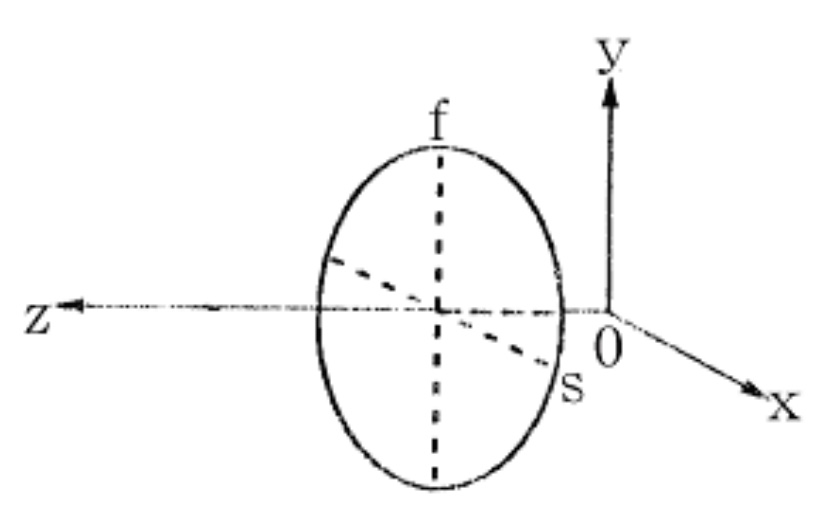
\includegraphics[width=0.26\textwidth]{/Users/kiloverse/Documents/物理学実験2/光の偏光/report_fig/位相差導き.jpg}} % 插入图片,并设置图片宽度为页面宽度的 38%(略小于图片区域占据的宽度,以留出一点间距)
        \caption{位相差板[1]}
        \label{fig:2}
    \end{wrapfigure}
    f軸方向とs軸方向の直線偏光波が同位相で、厚さのある位相差板に入射する場合、
    通過した $E_x$ と $E_y$ が一定の位相差が生じる。
    $z = 0$のときの位相を$\theta_f = \theta_s$と置くと、
    $z = d$での電場は以下と表せる。
\begin{equation}
    \mathbb{E}(d, t)=\hat{x} E_x \cos \left(\omega t-k_s d+\theta_s\right)+\hat{y} E_y \cos \left(\omega t-k_f d+\theta_f\right) \notag\\
\end{equation}
また、波数の定義より
\begin{align*} % 每行公式默认不带编号。
    & k_s=\frac{2 \pi}{\lambda_s}=\frac{2 \pi}{T} \cdot \frac{T}{\lambda_s}=\omega \cdot \frac{1}{v_s}=\omega \cdot \frac{n_s}{c} \\
    & \therefore k_s \cdot d=n_s \frac{\omega}{c} d, \quad k_f \cdot d=n_f \frac{\omega}{c} d 
\end{align*}
よって、電場と位相差は以下となる。
\begin{align*} % 每行公式默认不带编号。
    \mathbb{E}(d, t)&=\hat{x}_s E_s \cos \left(\omega t-n_s \frac{\omega}{c} d+\theta_s\right)+\hat{y} E_f \cos \left(\omega t-n_f \frac{\omega}{c} d+\theta_f\right) \\
    \Delta&=\left(n_s-n_f\right) \frac{\omega}{c} d 
\end{align*}

\begin{flushright} % 证毕符号
    $\qed$
\end{flushright}

\end{spacing}

\subsection{偏光状態}
\begin{spacing}{1.2} % 开始一个有首行缩进的段落,{自定义行间距}
    \noindent % 在特定段落前取消首行缩进
    偏光状態とは、光の波動が特定の方向に制限された振動を示す状態を指す。主に以下の三種類がある:
    \begin{itemize}
        \item 直線偏光:直線偏光は、電場ベクトルが一定の平面内で直線的に振動する状態で、光が特定の方向にのみ振動するということを意味する。
        \item 円偏光:円偏光では、電場ベクトルの振動が時間に対して一定の角度で円を描くように回転し続けることが特徴である。
        \item 楕円偏光:楕円偏光は、直線偏光と円偏光の中間の形をしていて、電場の振動が二つの直交成分の振幅や位相の差により楕円形を形成することにより生じる。
    \end{itemize}

    \noindent
    以上によって、偏光状態は位相差$\Delta$によって違う。
    \begin{equation}
        \begin{gathered}
        x \equiv \frac{E_x}{E_0}=\cos \omega t \\
        y \equiv \frac{E_y}{E_0}=\cos (\omega t+\Delta) \notag
        \end{gathered}
    \end{equation}
    とおいて、$t$を消去すると、
    \begin{equation}
        x^2-2 x y \cos \Delta+y^2=\sin ^2 \Delta \notag
    \end{equation}
    よって、$\Delta = n\pi$ のとき、$x = \pm y$ で、直線偏光となる。
    $\Delta = \pi/2 + n\pi$ のとき、$x^2 + y^2 = 1$ で、直線偏光となる。
    それ以外の場合、つまり$\Delta \not= n\pi/2$ のとき楕円偏光が生じる。
\end{spacing}

\subsection{直交$\cdot$平行ニコルにおける光強度}
\begin{spacing}{1.2}
    今回の実験2と実験Aでは、それぞれ直交ニコル法と平行ニコル法が用いられた。
    直交ニコル法では、偏光子と検光子を直交と設定し、その間に差し込んだ位相差板の光学的性質を調べることを可能とされた。
    それに対して、平行ニコル法では、偏光子と検光子の透過軸を平行と設定することとなっている。
    また、位相差を$\Delta$、偏光子と検光子の透過軸のなす角度を$\theta$とすると、
    直交ニコルと平行ニコルにおける光強度はそれぞれ式(3)と式(4)に従う。
    \begin{equation}
        I(\theta) = I_0 \sin^2(2\theta) \sin^2\left(\frac{\Delta}{2}\right)
    \end{equation}
    \begin{equation}
        I(\theta) = I_0 \left[ 1 - \sin^2(2\theta) \sin^2\left(\frac{\Delta}{2}\right) \right]
    \end{equation}
\end{spacing}

\subsubsection*{導き過程[2]}
\begin{spacing}{1.2}
    偏光子の透過軸の角度を$0$、位相差板の回転角を$\theta$、検光子の透過軸の角度を$\beta$、偏光子と検光子の透過軸のなす角度を$\alpha$とすると、
    位相差板から出射したx方向とy方向の電場の検光子透過軸方向の成分はそれぞれ以下となる: 
    \begin{align*}
        E_x &= E_i e^{i(\omega t - kz)} \cdot \cos{\theta} \cos{\beta}\\
        E_y &= E_i e^{i(\omega t - kz + \Delta)} \cdot \sin{\theta} \sin{\beta}
    \end{align*}
    よって、合成した電場の大きさは:
    \begin{align*}
        E_t &= E_i \left(\cos{\theta}\cos{\beta} + \sin{\theta}\sin{\beta}e^{i\Delta}\right)e^{i(\omega t - kz)}
    \end{align*}
    であり、二乗して光強度を計算すると、
    \begin{align*}
        |E_t|^2 &= E_i^2 \left[(\cos{\theta}\cos{\beta})^2 + (\sin{\theta}\sin{\beta})^2 + 2\cos{\theta}\cos{\beta}\sin{\theta}\sin{\beta}\cos{\Delta}\right] \\
                &= E_i^2 \left[(\cos{\theta}\cos{\beta})^2 + (\sin{\theta}\sin{\beta})^2 + 2\cos{\theta}\cos{\beta}\sin{\theta}\sin{\beta}(1 - 2 \sin^2{\Delta / 2})\right] \\
                &= E_i^2 \left[(\cos{\theta}\cos{\beta})^2 + (\sin{\theta}\sin{\beta})^2 + 2\cos{\theta}\cos{\beta}\sin{\theta}\sin{\beta} \right. \\
                &\qquad \left. - 4 \cos{\theta}\cos{\beta}\sin{\theta}\sin{\beta}\sin^2{\Delta/2}\right] \\ % \left. 表示开始但不显示左括号,使用 \right. 表示结束但不显示右括号
                &= E_i^2 \left[\cos^2{(\theta - \beta)} - \sin{2 \theta}\sin{2 \beta}\sin^2{\Delta/2}\right]
    \end{align*}
    が得られる。よって、直交ニコルにおいて、$\beta - \theta = \alpha = \pi/2$であるから、
    直交ニコルにおける光強度は以下となる:
    \begin{equation}
        I(\theta) = I_0 \sin^2(2\theta) \sin^2\left(\frac{\Delta}{2}\right) \notag
    \end{equation}
    平行ニコルにおいて、$\beta - \theta = \alpha = 0$であるから、
    平行ニコルにおける光強度は以下となる:
    \begin{equation}
        I(\theta) = I_0 \left[ 1 - \sin^2(2\theta) \sin^2\left(\frac{\Delta}{2}\right) \right] \notag
    \end{equation}
    \begin{flushright} % 证毕符号
        $\qed$
    \end{flushright}
\end{spacing}

% 3、実験手法%%%%%%%%%%%%%%%%%%%%%%%%%%%%%%%%%%%%%%%%%%%%%%%%
\section{実験手法}
\subsection{実験装置}
\begin{spacing}{1.2}
    本実験には、光源(ハロゲンランプ)、偏光子、位相差板、検光子、光検出器から成る基本的な光学系が用いられた。
    光源からの光が偏光子によって特定の偏光方向を持つ光に変換される。
    その後、位相差板を通過することで偏光状態が変化し、検光子を経て光検出器で光の強度が検出される。
    このセットアップ(図3)を基に、5つの実験が行われた。
\end{spacing}
\begin{figure}[!htb] % 选项 [htbp] 代表位置优先级, “here, top, bottom, page” 分别表示:此处、页顶、页底、单独一页
    \centering
    \fbox{\adjincludegraphics[width=0.618\textwidth, keepaspectratio]{/Users/kiloverse/Documents/物理学実験2/光の偏光/report_fig/実験装置.JPG}}
    \caption{実験装置}
    \label{fig:3}
\end{figure}
\FloatBarrier

\subsection{実験方法[3]}
\subsubsection{実験1}
\begin{spacing}{1.2}
    \noindent % 在特定段落前取消首行缩进
    マリュスの法則を検証するため、2枚のポラロイド(偏光子と検光子)を使って、
    その相対角を変化させながら、光の強度を測定し、理論との一致を確認した。
    (本実験では便宜上に、偏光子を0目盛りに固定し、検光子だけを回し、目盛りの差から相対角を獲得した。)
\end{spacing}

\subsubsection{実験2 $\cdot$ 実験A}
\begin{spacing}{1.2}
    \noindent % 在特定段落前取消首行缩进
    実験2では、偏光子と検光子の透過軸を垂直と設定し、
    その間に位相差板を差し込んで、光強度の位相差板角度の依存性を調べた(直交ニコル法)。
    それに対して、実験Aでは、偏光子と検光子の透過軸を平行と設定し、
    位相差板を回しながら、光強度を測った(平行ニコル法)。
\end{spacing}

\subsubsection{実験3 $\cdot$ 実験B}
\begin{spacing}{1.2}
    \noindent % 在特定段落前取消首行缩进
    実験3と実験Bでは位相差板を用いて楕円偏光が生成された。
    実験3では、偏光子と検光子が直交する配置において、
    透過光強度が最大のところに位相差板を固定し、
    検光子を回転させて、角度ごとの光強度を測った。
    実験Bでは実験3と違う位相差板角度の下で、光強度の検光子角度の依存性を調べた。
    (具体的には、実験3の透過光強度が最大のところを位相差板の45度として、30度$\cdot$15度$\cdot$0度に位相差板を固定し、
    検光子を回転させて、角度ごとの光強度のデータを取った。)
    以上の実験から生じる楕円偏光の特性を解析した。
\end{spacing}

% 4、実験結果%%%%%%%%%%%%%%%%%%%%%%%%%%%%%%%%%%%%%%%%%%%%%%%%
% \section{実験結果}

% 5、実験考察%%%%%%%%%%%%%%%%%%%%%%%%%%%%%%%%%%%%%%%%%%%%%%%%
\section{実験結果 $\cdot$ 考察}
\subsection{実験1}
\subsubsection{結果}
\begin{spacing}{1.2}
    図4は実測データと$I_0cos^2\theta$の比較で、
    図5は光強度の角度ごとのレーザー図である。
    (ただじ、横軸の$\theta$は、偏光子と検光子の透過軸のなす角度ではなく、検光子自体の回転角度である)
\end{spacing}

\begin{figure}[htbp]
    \centering
    \begin{minipage}[b]{0.5\textwidth} % minipage 环境用于在同一行内并排放置内容,[b] 参数表示底部对齐,{0.5\textwidth} 设置 minipage 的宽度为页面宽度的一半
      \centering
      \adjustbox{height=0.23\textheight,keepaspectratio}{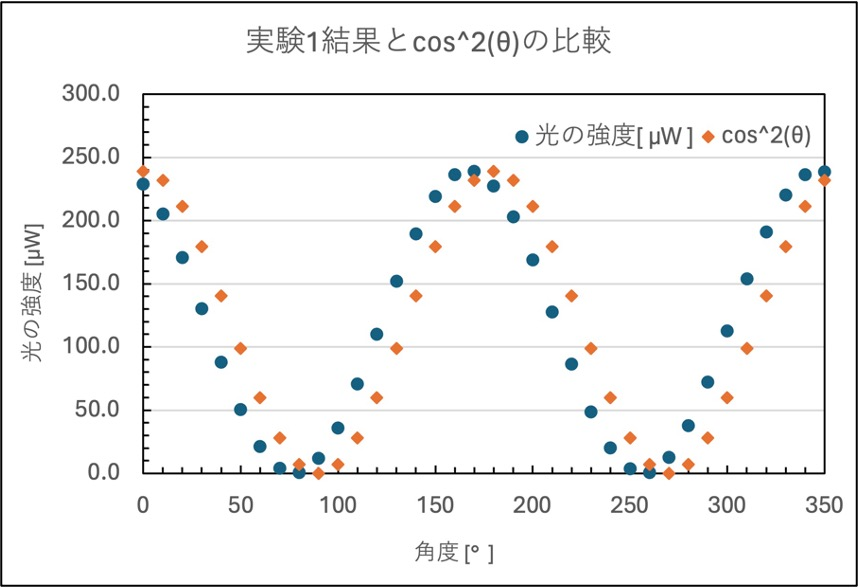
\includegraphics{/Users/kiloverse/Documents/物理学実験2/光の偏光/report_fig/実験1光強度(fitting前).jpg}} % 使用 \adjustbox 命令将图片高度设置为 0.3\textheight,根据需要调整 height 参数,以确保图片的高度合适
      \caption{実験1:光強度と検光子角度の関係}
      \label{fig:4}
    \end{minipage}% % 在两个 minipage 环境之间使用 % 符号来消除之间的空白
    \begin{minipage}[b]{0.5\textwidth}
      \centering
      \adjustbox{height=0.23\textheight,keepaspectratio}{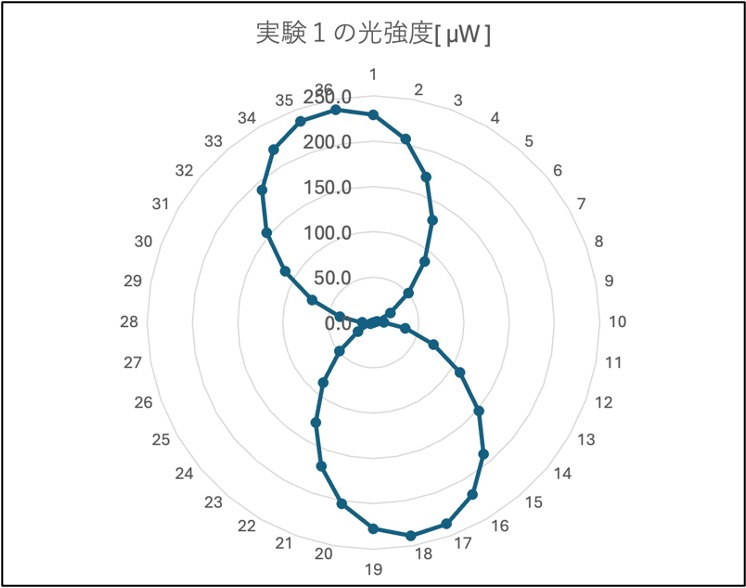
\includegraphics{/Users/kiloverse/Documents/物理学実験2/光の偏光/report_fig/実験1レーザー.jpg}}
      \caption{実験1:角度ごとの光強度レーザー図}
      \label{fig:5}
    \end{minipage}
\end{figure}
\FloatBarrier

\subsubsection*{結果の解析}
\begin{spacing}{1.2}
    実験結果のデータは、理論曲線$I_0cos^2\theta$と比較されたが、
    データには理論曲線との間にわずかなずれが見られた。
    このずれの原因は、検光子の透過軸が0度の目盛りに完全に合っていないためである。
    しかし、データの形状が理論曲線と一致していることから、
    マリュスの法則が実験を通じて確認された。
    これは、光の強度が相対角の余弦の二乗に依存することを示しており、法則の有効性を裏付ける結果である。
\end{spacing}

\subsubsection{考察}
\begin{spacing}{1.2}
    検光子の透過軸が0度の目盛りではないことから生じたデータと理論曲線の間のずれを修正するために、
    最小二乗法を用いたフィッティングプログラムを書いて、偏光子の実際の位置を特定するパラメータを求めることを試みった。
    検光子角度$\theta$にある角度$\alpha$を足して、
    理論曲線$I_0cos^2\theta$と実測データとの間の差の二乗和を最小化させるようにフィッティングした。
    具体的なコードは以下となる:
\end{spacing}

\begin{lstlisting} 
import numpy as np
from scipy.optimize import minimize

# 実測データ
theta = np.array([0, 10, 20, 30, 40, 50, 60, 70, 80, 90, 100, 110, 120, 130, 140, 150, 160, 170, 180, 190, 200, 210, 220, 230, 240, 250, 260, 270, 280, 290, 300, 310, 320, 330, 340, 350])
intensity = np.array([229, 205.4, 170.8, 130.2, 88.1, 50.7, 21.4, 4.2, 0.6, 11.8, 35.9, 70.7, 110.1, 152, 189.4, 219.2, 236.4, 239.1, 227.5, 202.9, 168.8, 127.7, 86.3, 48.8, 20, 3.54, 0.8, 12.7, 37.7, 72.4, 112.8, 154.1, 191.1, 220.4, 236.3, 238.6])

def calc_error(alpha):
    rad = np.radians(theta + alpha)  # 角度をradに変換し、alphaを加算
    cos_squared = np.cos(rad)**2 * 239.1  # cos^2(theta + alpha) を計算
    error = np.sum((cos_squared - intensity)**2)  # 誤差の平方和
    return error

result = minimize(calc_error, x0=0)  # 初期値として alpha = 0 を使用
best_alpha = result.x  # 最適な alpha を取得

print("the best alpha = ", best_alpha)
\end{lstlisting}

\begin{spacing}{1.2}
    \indent % 在特定段落前取消首行缩进
    以上を実行してみると、Outputは
\end{spacing}

\begin{lstlisting} 
    the best alpha =  [12.93014215]
\end{lstlisting}

\begin{spacing}{1.2}
    \noindent % 在特定段落前取消首行缩进
    となった。よって、検光子の透過軸の位置は凡そ目盛りの$-12.93$
    (つまり、$360-12.93 = 347.07$)のところにあると考察する。
    これはレーザー図からも予想できる。
    レーザー図(図6)において、光強度の分布は明らかに傾いている。
    その傾いた角度は約$-13$度で、フィッティングの結果と合っている。\\
    また、レーザー図に2本の羽根が見えるのは、
    光強度が360度において2周期があることを意味している。
    それもマリュスの法則の式$I(\theta) = I_0cos^2\theta$と一致している。
    \begin{figure}[htbp]
        \centering
        \begin{minipage}[b]{0.5\textwidth} % minipage 环境用于在同一行内并排放置内容,[b] 参数表示底部对齐,{0.5\textwidth} 设置 minipage 的宽度为页面宽度的一半
          \centering
          \fbox{\adjustbox{height=0.23\textheight,keepaspectratio}{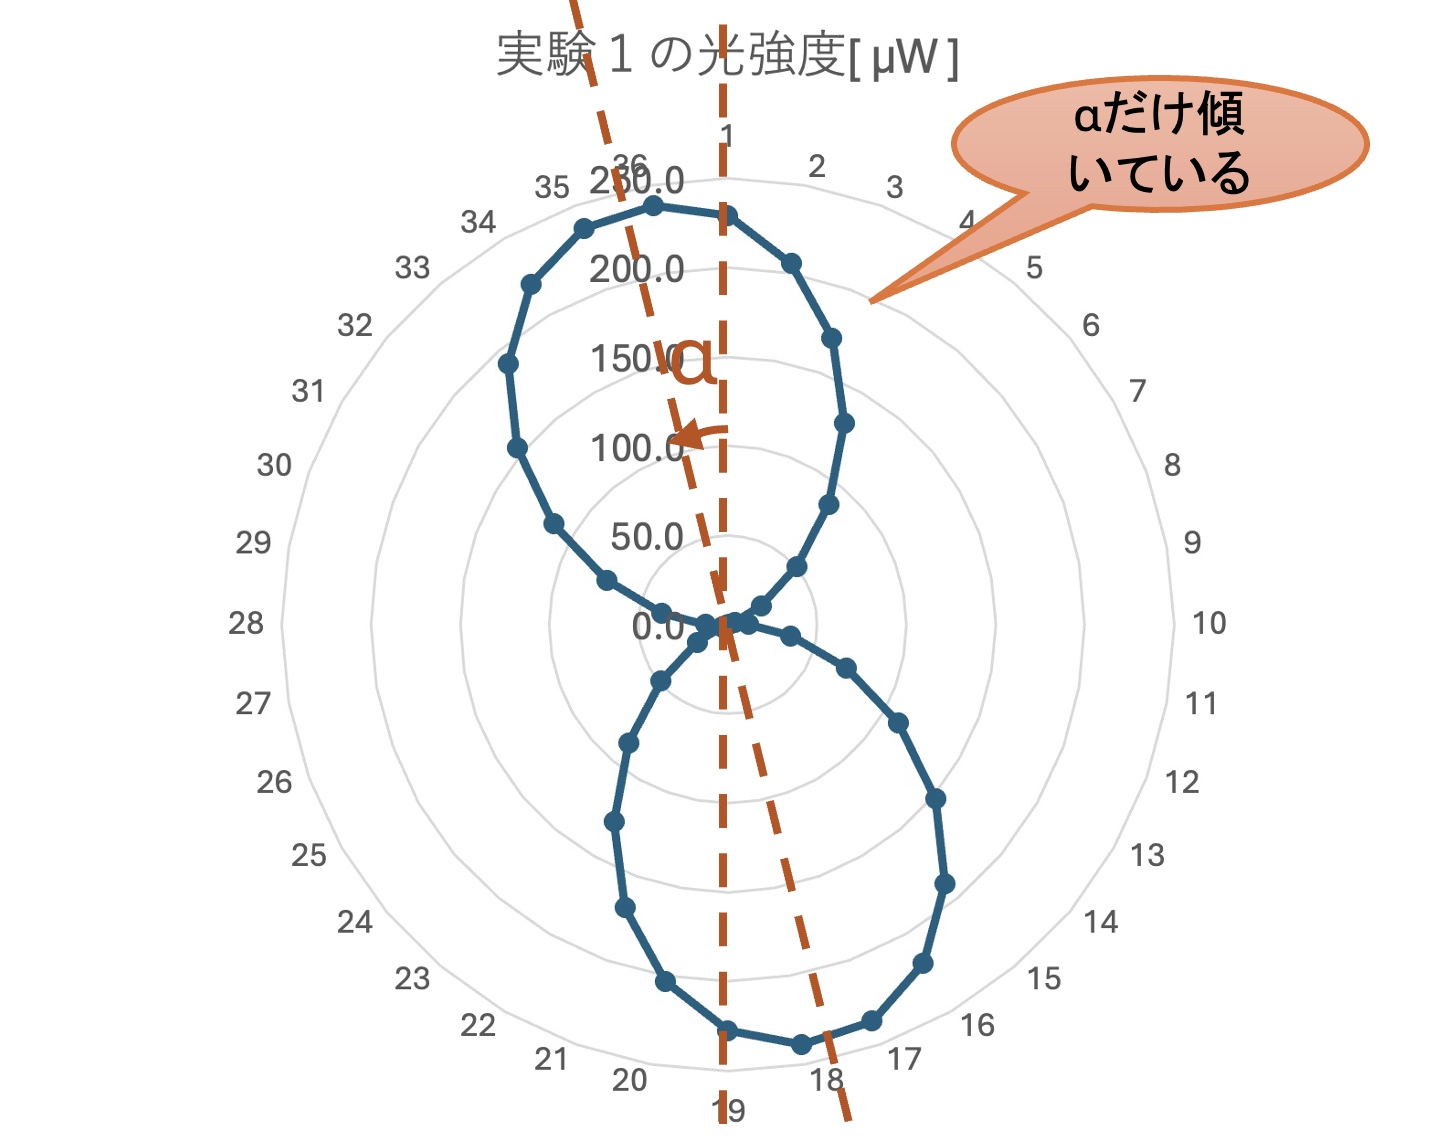
\includegraphics{/Users/kiloverse/Documents/物理学実験2/光の偏光/report_fig/実験1レーザー図考察.JPG}}} % 使用 \adjustbox 命令将图片高度设置为 0.3\textheight,根据需要调整 height 参数,以确保图片的高度合适
          \caption{レーザー図の傾き角と形の考察}
          \label{fig:6}
        \end{minipage}% % 在两个 minipage 环境之间使用 % 符号来消除之间的空白
        \begin{minipage}[b]{0.5\textwidth}
          \centering
          \fbox{\adjustbox{height=0.23\textheight,keepaspectratio}{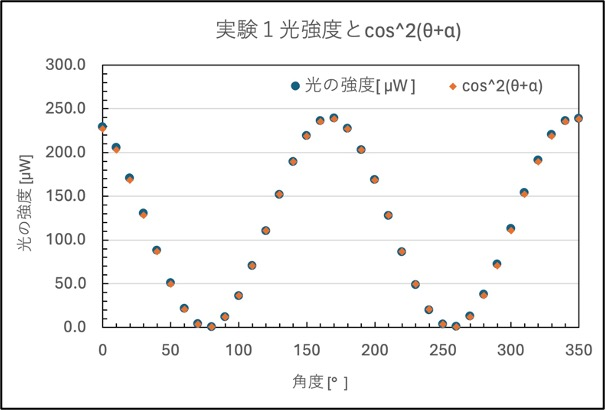
\includegraphics{/Users/kiloverse/Documents/物理学実験2/光の偏光/report_fig/実験1fitting後.jpg}}} % 使用 \adjustbox 命令将图片高度设置为 0.3\textheight,根据需要调整 height 参数,以确保图片的高度合适
          \caption{再プロットした結果}
          \label{fig:7}
        \end{minipage}
    \end{figure}
    \FloatBarrier
    改めて実測データと修正した理論曲線$I_0cos^2(\theta + \alpha)$を再プロットすると、
    図7の通りに、理論曲線と実測データとの間の一致が顕著に改善された。
    よって、マリュスの法則が検証された。
\end{spacing}

\subsection{実験2 $\cdot$ 実験A}
\subsubsection{結果}
\begin{spacing}{1.2}
    図8は直交ニコル法を使った実験2で得た光強度の位相差板角度による分布で、
    図9は実験2の光強度の位相差板角度ごとのレーザー図である。
\end{spacing}
\begin{figure}[htbp]
    \centering
    \begin{minipage}[b]{0.5\textwidth} % minipage 环境用于在同一行内并排放置内容,[b] 参数表示底部对齐,{0.5\textwidth} 设置 minipage 的宽度为页面宽度的一半
      \centering
      \adjustbox{height=0.23\textheight,keepaspectratio}{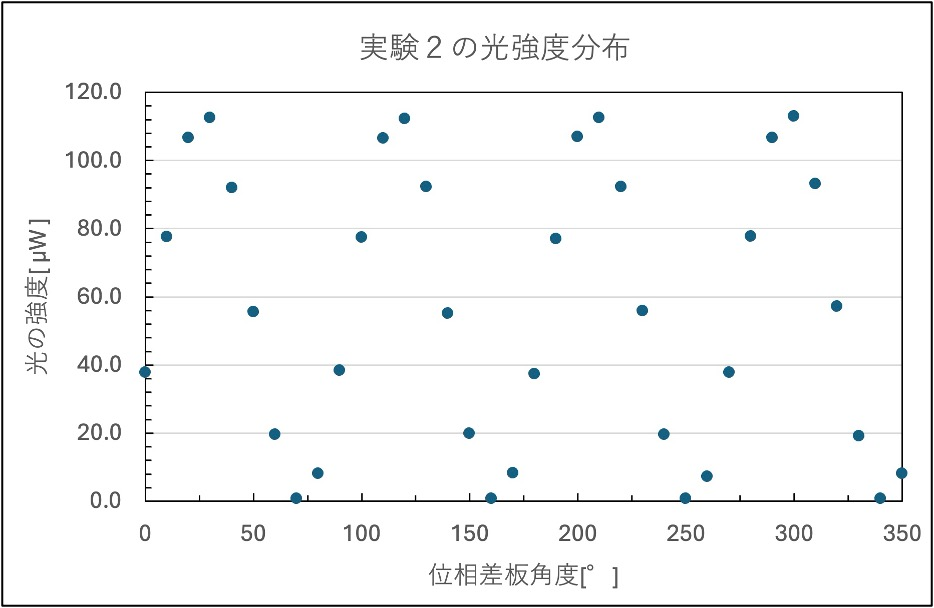
\includegraphics{/Users/kiloverse/Documents/物理学実験2/光の偏光/report_fig/実験2光強度.jpg}} % 使用 \adjustbox 命令将图片高度设置为 0.3\textheight,根据需要调整 height 参数,以确保图片的高度合适
      \caption{実験2:光強度と位相差板角度の関係}
      \label{fig:8}
    \end{minipage}% % 在两个 minipage 环境之间使用 % 符号来消除之间的空白
    \begin{minipage}[b]{0.5\textwidth}
      \centering
      \adjustbox{height=0.23\textheight,keepaspectratio}{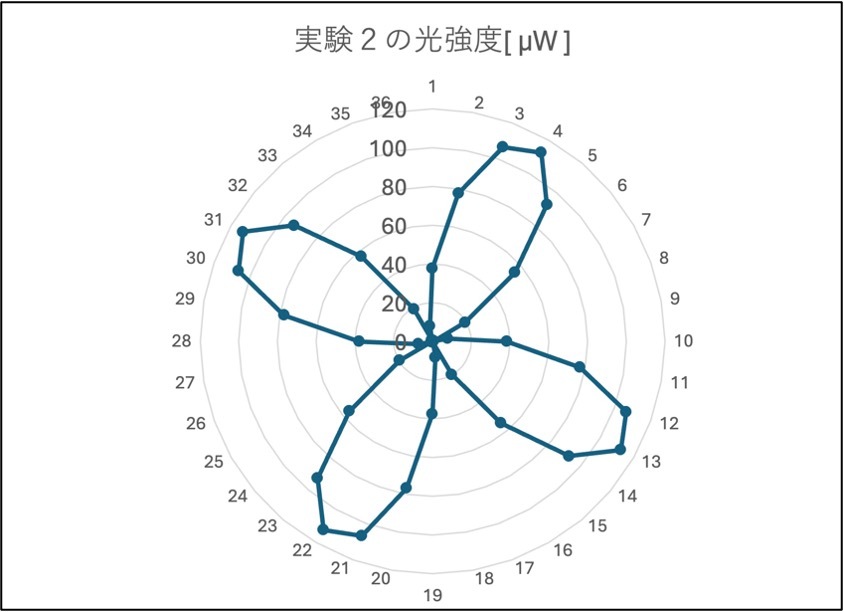
\includegraphics{/Users/kiloverse/Documents/物理学実験2/光の偏光/report_fig/実験2レーザー.jpg}}
      \caption{実験2:角度ごとの光強度レーザー図}
      \label{fig:9}
    \end{minipage}
\end{figure}
\FloatBarrier

\begin{spacing}{1.2}
    図10は平行ニコル法を使った実験Aで得た光強度の位相差板角度による分布で、
    図11は実験Aの光強度の位相差板角度ごとのレーザー図である。
\end{spacing}
\begin{figure}[htbp]
    \centering
    \begin{minipage}[b]{0.5\textwidth} % minipage 环境用于在同一行内并排放置内容,[b] 参数表示底部对齐,{0.5\textwidth} 设置 minipage 的宽度为页面宽度的一半
      \centering
      \adjustbox{height=0.23\textheight,keepaspectratio}{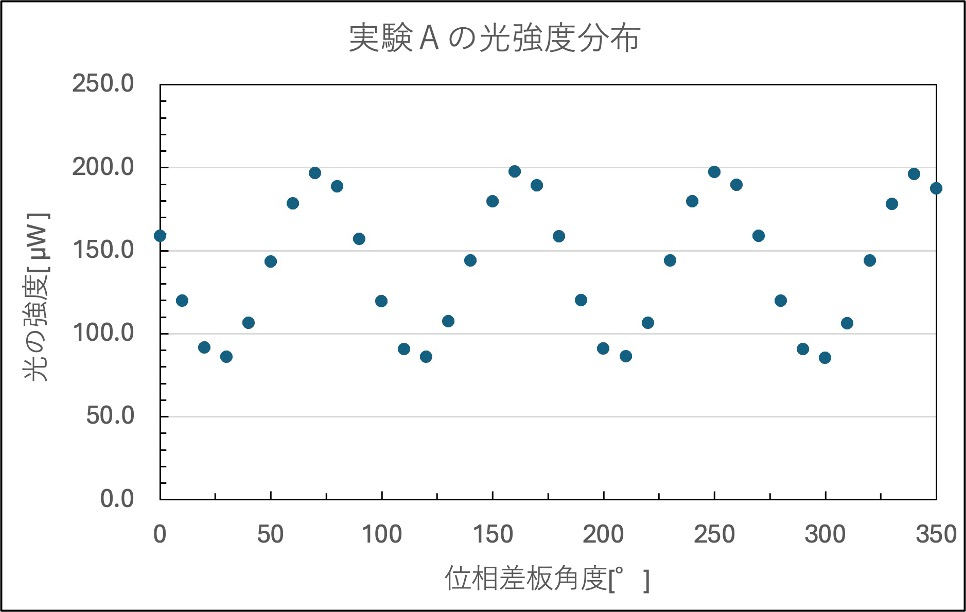
\includegraphics{/Users/kiloverse/Documents/物理学実験2/光の偏光/report_fig/実験A光強度.jpg}} % 使用 \adjustbox 命令将图片高度设置为 0.3\textheight,根据需要调整 height 参数,以确保图片的高度合适
      \caption{実験A:光強度と位相差板角度の関係}
      \label{fig:10}
    \end{minipage}% % 在两个 minipage 环境之间使用 % 符号来消除之间的空白
    \begin{minipage}[b]{0.5\textwidth}
      \centering
      \adjustbox{height=0.23\textheight,keepaspectratio}{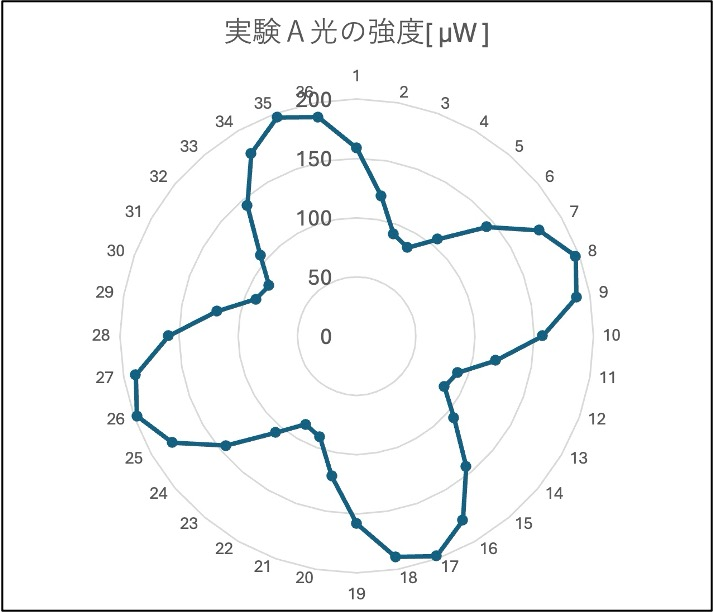
\includegraphics{/Users/kiloverse/Documents/物理学実験2/光の偏光/report_fig/実験Aレーザー.jpg}}
      \caption{実験A:角度ごとの光強度レーザー図}
      \label{fig:11}
    \end{minipage}
\end{figure}
\FloatBarrier

\subsubsection*{結果の解析}
\begin{enumerate}[label=\arabic*), before=\begin{spacing}{1.2}, after=\end{spacing}] % \arabic阿拉伯数字,\roman小写罗马数字,\Roman,\alph小写字母,\Alph,“*”之后添加自己喜欢的序号后样式, 如1.添加“.”,1)添加“)”;利用{spacing}自定义\item内的行间距
    \item 実験2の解析: \\
    実験2では直交ニコル法が用いられ、
    偏光子と検光子の透過軸が垂直に設定された。
    理論的には、位相差板がなければ光強度はゼロになるはずである。
    しかし、位相差板を挿入したことで、
    光の電場成分がX方向とY方向で位相差を生じ、
    これが合成された偏光状態が変化するため、光強度がゼロではなくなる[4]。
    実測データのレーザー図は、
    この位相差の影響を受けて閉じる(クロス)パターンを示しており、
    位相差の光軸において、光強度がゼロであり、
    偏光方向が元の偏光子の透過軸方向から変化したことが観察される。
    \begin{figure}[!htb] % 选项 [htbp] 代表位置优先级, “here, top, bottom, page” 分别表示:此处、页顶、页底、单独一页
        \centering
        \fbox{\adjincludegraphics[width=0.618\textwidth, keepaspectratio]{/Users/kiloverse/Documents/物理学実験2/光の偏光/report_fig/実験2位相差板考察引用図.jpg}}
        \caption{位相差板による偏光方向の変化[4]}
        \label{fig:12}
    \end{figure}
    \FloatBarrier
    \item 実験Bの解析: \\
    一方、実験Aでは平行ニコル法が採用され、
    偏光子と検光子の透過軸が平行に設定された。
    位相差板を回しながら光強度を測定すると、
    位相差板が光の偏光状態を変えるために、光強度は周期的に変化し、
    しかし基本的には透過光が存在する。
    よって、実験Aのレーザー図は開いている(オープン)パターンを示し、
    光強度がゼロのなる角度は存在しない。
    \item 実験2と実験Aの比較
    実験2の結果は、位相差板が偏光方向を変更する効果を示し、
    直交ニコル設定においても完全な光の遮断が行われなかったことを示している。
    これに対し、実験Aでは、位相差板の回転によって偏光方向が連続的に変化し、
    偏光子と検光子が平行の場合においても光強度が周期的に増減する様子が確認された。
    この二つの実験から、位相差板が偏光状態に与える影響の程度とそのメカニズムの理解が深まった。
\end{enumerate}

\subsubsection{考察}
\subsubsection*{実験2の考察}
\begin{spacing}{1.2}
    実験2における実測データが理論式と一致しているかどうかを評価し、
    位相差板の光軸の位置及びそれによる位相差を特定するように、
    以下のフィッティングプログラムを作成した。
\begin{lstlisting}
import numpy as np
import matplotlib.pyplot as plt
from scipy.optimize import curve_fit

# 実測データ
theta_deg = np.array([0, 10, 20, 30, 40, 50, 60, 70, 80, 90, 100, 110, 120, 130, 140, 150, 160, 170, 180, 190, 200, 210, 220, 230, 240, 250, 260, 270, 280, 290, 300, 310, 320, 330, 340, 350])
intensity = np.array([37.8, 77.6, 106.7, 112.5, 92, 55.5, 19.6, 0.8, 8.1, 38.4, 77.4, 106.5, 112.2, 92.2, 55.1, 19.8, 0.7, 8.3, 37.4, 77, 106.9, 112.5, 92.2, 55.9, 19.5, 0.7, 7.3, 37.8, 77.8, 106.6, 113, 93.1, 57.2, 19.2, 0.7, 8.1])

# 角度を rad に変換 
theta_rad = np.deg2rad(theta_deg)

# 直交ニコルの理論式
def theoretical_intensity(theta, I_0, alpha, delta): 
    theta = theta + alpha # 位相差板の光軸の位置をfitするために alpha を加算
    return I_0 * np.sin(2 * theta)**2 * np.sin(delta / 2)**2

# fitting
popt, pcov = curve_fit(theoretical_intensity, theta_rad, intensity, p0 = [239.1, 0, np.pi/2]) # 実験1で測定した光強度の最大値を光源強度の初期値とする
I_0_fit, alpha_fit, delta_fit = popt

# fitting結果を output
print("I_0 = ", I_0_fit)
print("alpha_rad = ", alpha_fit)
print("alpha_deg = ", np.rad2deg(alpha_fit))
print("delta_rad = ", delta_fit)
print("delta_deg = ", np.rad2deg(delta_fit))
\end{lstlisting}
    このプログラムは、位相差板角度にある角度を加えることで、
    位相差板の光軸の位置を推定しようとするものである。
    具体的には、curve fit を用いて実測データと直交ニコルの理論式
    $I(\theta) = I_0 \sin^2(2\theta) \sin^2\left(\Delta / 2\right)$
    が最も一致するようなパラメータを求めることにより、
    最適なパラメータを求めてみた。
    実行してみたら、出力は以下となった。
\begin{lstlisting}
    I_0 =  215.9290762993863         # 最適な光源強度
    alpha_rad =  0.30967416906518547 # 最適な位相差板の光軸位置(rad)
    alpha_deg =  17.743022911655846  # 最適な位相差板の光軸位置(deg)
    delta_rad =  1.6233710320344104  # 最適な位相差(rad)
    delta_deg =  93.01230871936848   # 最適な位相差(deg)
\end{lstlisting}
フィッティングプログラムによって得られたパラメータを用いて、
理論式と実測データの一致性を評価するために、
次の手順で計算およびプロットを行った。
\begin{lstlisting}
# fitting結果を用いて理論値を計算
theta_fit = np.linspace(0, 2 * np.pi, 500)
intensity_fit = theoretical_intensity(theta_fit, I_0_fit, alpha_fit, delta_fit)
    
# プロット
plt.figure(figsize = (10, 6))
plt.plot(np.rad2deg(theta_fit), intensity_fit, label = 'theoretical intensity')
plt.scatter(theta_deg, intensity, color = 'red', label = 'experimental intensity')
plt.xlabel('theta [degree]')
plt.ylabel('Intensity [ $\mu W$]')
plt.title('Fitted Theoretical I vs Experimental I (close nicol)')
plt.legend()
plt.grid(True)
plt.show()
\end{lstlisting}

    \noindent
    プロットの結果は以下の図13通りである:

\begin{figure}[!htb] % 选项 [htbp] 代表位置优先级, “here, top, bottom, page” 分别表示:此处、页顶、页底、单独一页
    \centering
    \fbox{\adjincludegraphics[width=0.618\textwidth, keepaspectratio]{/Users/kiloverse/Documents/物理学実験2/光の偏光/report_fig/実験2_Malplotbib.png}}
    \caption{実験2のフィッティング結果}
    \label{fig:13}
\end{figure}
\FloatBarrier
    以上のフィッティング結果について考察していくと、
    $\alpha$が約18度であることから、
    位相差板の光軸の位置は実際の角度目盛りで342度(360度 - 18度)
    の位置にあると推測される。
    また、$\Delta$が93°$\approx \pi/2$であることは、
    X方向とY方向の電場成分間にの約 $\pi/2$ の位相差が生じて、
    今回の実験に用いられたのは1/4位相差板だとと示唆するが、
    その妥当性は後の実験2 $\cdot$ の部分でまた考察する。
    それに、Matplotlibで描かれた図を通じて、
    理論モデルと実験データが良好に一致していることが確認できた。
    この一致は、実験のセットアップが適切であり、
    測定データの質が高いことを示唆している。
\end{spacing}

\subsubsection*{実験Aの考察}
\begin{spacing}{1.2}
    実験Aでは、位相差板の光軸位置と位相差を求めるために、
    実験2と同様に、
    実測データと平行ニコルの理論式
    $I(\theta) = I_0 \left[ 1 - \sin^2(2\theta) \sin^2\left(\Delta / 2\right) \right]$
    が最も一致するようフィッティングプログラムを作成した。
    (プログラムのアルゴリズムは実験2とほぼ同じで、
    詳細はここでは略するが、コードの全文は文末の付録に記載されている。)
    フィッティングの結果は以下となった。
    \begin{lstlisting}
    I_0 =  197.51909945881744
    alpha_rad =  0.3157245136513319
    alpha_deg =  18.089682121041864
    delta_rad =  1.427356365582847
    delta_deg =  81.78149560902932
    \end{lstlisting}
    \begin{figure}[!htb] % 选项 [htbp] 代表位置优先级, “here, top, bottom, page” 分别表示:此处、页顶、页底、单独一页
        \centering
        \fbox{\adjincludegraphics[width=0.618\textwidth, keepaspectratio]{/Users/kiloverse/Documents/物理学実験2/光の偏光/report_fig/実験A_Matlpotlib.png}}
        \caption{実験Aのフィッティング結果}
        \label{fig:14}
    \end{figure}
    \indent
    フィッティングの結果、
    初期強度$I_0$は約197.519、
    $\alpha$は約18度、
    $\Delta$は約82度求められた。
    これらのパラメータは、
    位相差板の光軸位置が実際の角度目盛りで342度(360度 - 18度)
    の位置にあることを示唆しており、位相差が約82度であることを示している。
    (実験2と異なる位相差の結果が得られた原因をは後でさらに詳細に考察する。)
    また、Matplotlibで描かれた図14から理論モデルと実験データが良好に一致していることが確認できたため、
    実験Aの手法とデータの質が有効であると評価される。
\end{spacing}

\subsubsection*{実験2と実験Aの比較}
\begin{spacing}{1.2}
    これからは実験2と実験Aを比較しながら、考察していきたいと思う。\\
    \indent
    まず、実験2のフィッティングより、入射光強度は215.9 $\mu W$と推測されたが、
    実験Aのフィッティングによる入射光強度は197.5 $\mu W$である。
    実際に、実験2と実験Aの実測データを比較してみると、
    図15通りに、実験2の光強度$I_2$の最大値は、
    実験Aの光強度$I_A$の最小値より大きくなっている。
    \begin{figure}[!htb] % 选项 [htbp] 代表位置优先级, “here, top, bottom, page” 分别表示:此处、页顶、页底、单独一页
        \centering
        \fbox{\adjincludegraphics[width=0.45\textwidth, keepaspectratio]{/Users/kiloverse/Documents/物理学実験2/光の偏光/report_fig/実験2plus実験A.JPG}}
        \caption{実験2と実験Aの光強度及びその加算}
        \label{fig:15}
    \end{figure}
    \FloatBarrier
    \noindent
    しかしながら、理論式
    \begin{align}
        I_2(\theta) &= I_0 \sin^2(2\theta) \sin^2\left(\frac{\Delta}{2}\right)\\
        I_A(\theta) &= I_0 \left[ 1 - \sin^2(2\theta) \sin^2\left(\frac{\Delta}{2}\right) \right]
    \end{align}
    によると、$Max(I_2) = Min(I_A)$ のはずである
    (なぜならば、$Max(I_2)$と$Min(I_A)$はともに
    $\sin^2(2\theta) \sin^2\left(\Delta/2\right)$が最大になる時にとる)。
    そのずれは、偏光子と検光子の設定が異なることによって、
    実験2と実験Aにおける光の吸収量が違うが原因だと考えられる。
    吸収量を影響する要因は以下検討する:
    \begin{itemize}
        \item 位相差板の配置が適切でない、
        または板自体に不均一性がある場合、
        光の位相変化に加えて吸収が発生することがある。
        \item 実験2と実験Aで検光子の角度が$\pi/2$変わったため、
        検光子の品質が不十分な場合、
        理論的な予測と異なる光の挙動が観察される可能性がある。
        特に、素材の内部での不純物や欠陥が光の吸収を増加させる原因となる。
        \item また、実験2 $\cdot$ 実験Aにおける光検出器の配置が異なる場合、
        あるいは光検出器が最適な位置にない場合、
        それぞれの実験で光の検出効率が変わり、
        理論値と実測値の間にズレが生じることが考えられる。
    \end{itemize}

    また、実験2のフィッティングから得られた位相差が 1.623 rad に対して
    実験Aから得られた位相差が 1.427 rad である。
    先に実験3の結論を使ってしまうと、
    今回の実験で使った位相差板の位相差は 1.280 rad ($0.41\pi$)だと推測された。
    その誤差の生じた原因はまた、
    光学系による光の吸収と関係あると推測する。

    そもそも理論式の $I_0$ は入射光の強度(光源強度)であるはずだが、
    それが未知であるため、フィッティングした時、
    検出された出射光強度を代入した。
    しかしながら、光が光学系を通過する際に、
    ある程度吸収されることがあるから、
    フィッティングで使ったデータは、
    入射光の強度 $I_0$ と違い値になっていて、
    最後の光強度と位相差のフィッティング結果に影響を及ぼす恐れがある。

    以上の推測を検証するために、
    フィッティングにおいて、
    $I_0$ にある通過率 $r$ をかけて、
    光の通過率 $r$ についてもフィッティングしてみると、
    実験2のアウトプット:
    \begin{lstlisting}
    I_0 =  254.85479449237076        # 最適な光源強度
    delta_rad =  1.5325199265495926  # 最適な位相差(rad)
    r =  0.9272712399872978          # 最適な光の通過率
    \end{lstlisting}
    実験Bのアウトプット:
    \begin{lstlisting}
    I_0 =  226.85100896193865        # 最適な光源強度
    delta_rad =  1.4273563655945756  # 最適な位相差(rad)
    r =  0.8706996735999267          # 最適な光の通過率
    \end{lstlisting}
    (プログラムの詳細は付録に記載された。)

    以上の結果より、
    $I_0$ にある通過率 $r$ をかけることで、
    光源強度 $I_0$ の精度が良くなった一方、
    推定された位相差と 1.280 rad の相対誤差も小さくなった。
    よって、光学系による吸収はフィッティング結果に影響があると確認できた。

    ただし、curve fit などのフィッティング手法を用いて、
    多くのパラメータを持つモデルで
    多くのパラメータを同時に推定する場合、
    そのパラメータがデータに与える影響が相互に依存している場合があって、
    個々のパラメータを正確に推定することが困難になり、
    フィッティング結果が安定しなかったり、
    パラメータ間でトレードオフが生じたりすることがある。
    今のように、無理にデータをフィッティングすることより、
    むしろ実験の時ちゃんと入射光強度のデータを取るの方が妥当だと思う。
\end{spacing}

\newpage
\subsection{実験3 $\cdot$ 実験B}
\subsubsection{結果}
\begin{spacing}{1.2}
    図16は実験3における光強度の検光子角度による分布で、
    図17はそのレーザー図である。
    \begin{figure}[htbp]
        \centering
        \begin{minipage}[b]{0.5\textwidth} % minipage 环境用于在同一行内并排放置内容,[b] 参数表示底部对齐,{0.5\textwidth} 设置 minipage 的宽度为页面宽度的一半
          \centering
          \adjustbox{height=0.23\textheight,keepaspectratio}{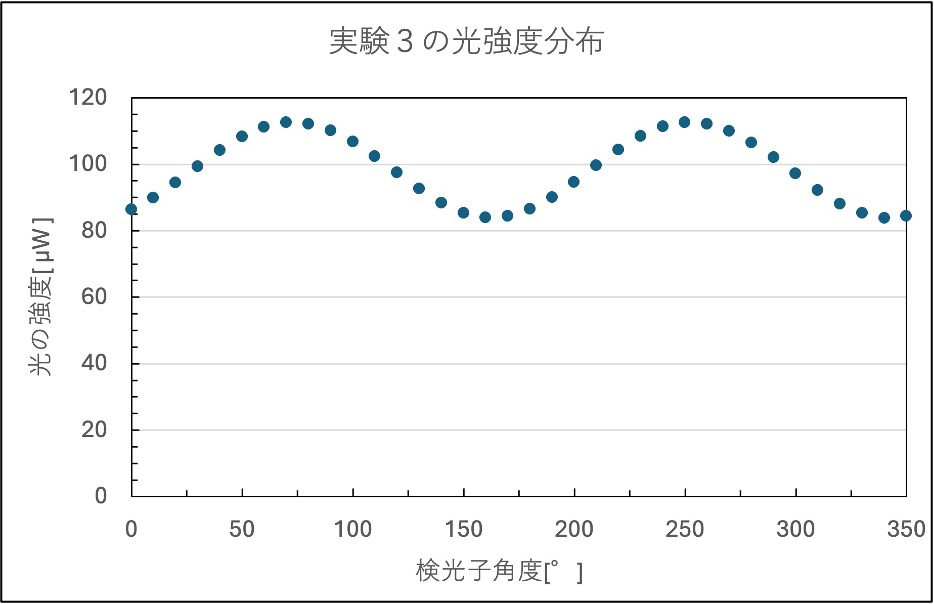
\includegraphics{/Users/kiloverse/Documents/物理学実験2/光の偏光/report_fig/実験3光強度.jpg}} % 使用 \adjustbox 命令将图片高度设置为 0.3\textheight,根据需要调整 height 参数,以确保图片的高度合适
          \caption{実験3:光強度と検光子角度の関係(45°)}
          \label{fig:16}
        \end{minipage}% % 在两个 minipage 环境之间使用 % 符号来消除之间的空白
        \begin{minipage}[b]{0.5\textwidth}
          \centering
          \adjustbox{height=0.23\textheight,keepaspectratio}{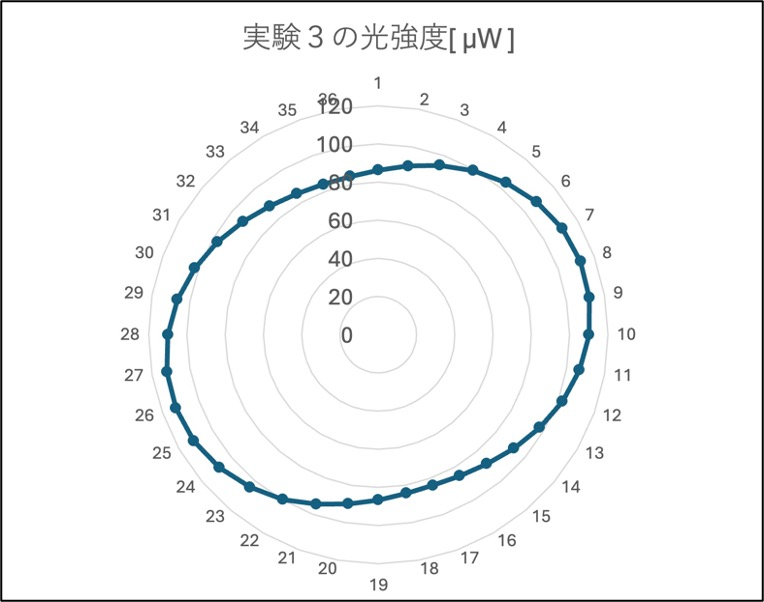
\includegraphics{/Users/kiloverse/Documents/物理学実験2/光の偏光/report_fig/実験3レーザー.jpg}}
          \caption{実験3:角度ごとの光強度レーザー図(45°)}
          \label{fig:17}
        \end{minipage}
    \end{figure}
    \FloatBarrier
    また、実験3の透過光強度が最大のところを位相差板の45度として、
    図18 $\cdot$図20 $\cdot$図22はそれぞれ、
    位相差板が30度 $\cdot$ 15度 $\cdot$ 0度の場合の
    光強度の検光子角度による分布である。
    図19 $\cdot$図21 $\cdot$図23はそれに対応するレーザー図である。
    \begin{figure}[htbp]
        \centering
        \begin{minipage}[b]{0.5\textwidth} % minipage 环境用于在同一行内并排放置内容,[b] 参数表示底部对齐,{0.5\textwidth} 设置 minipage 的宽度为页面宽度的一半
          \centering
          \adjustbox{height=0.23\textheight,keepaspectratio}{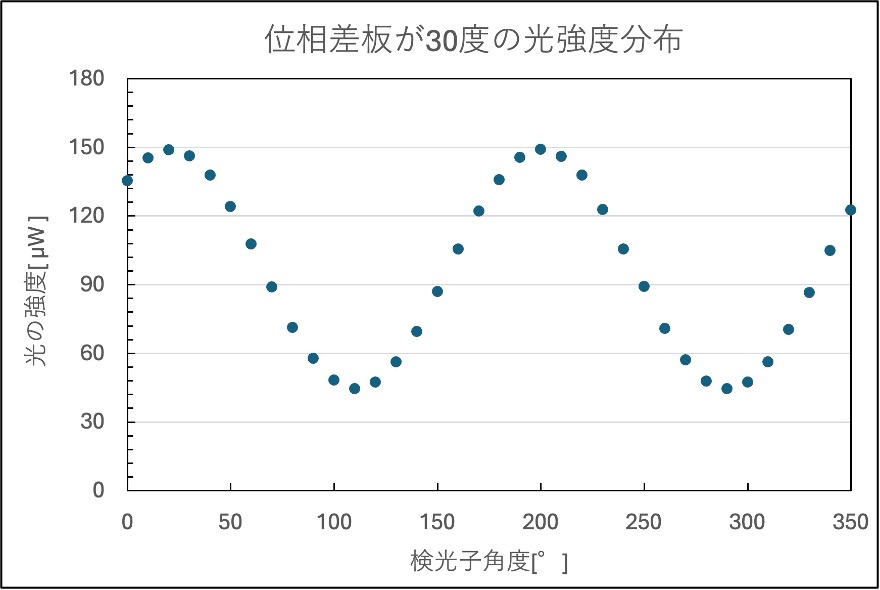
\includegraphics{/Users/kiloverse/Documents/物理学実験2/光の偏光/report_fig/実験B光強度30.jpg}} % 使用 \adjustbox 命令将图片高度设置为 0.3\textheight,根据需要调整 height 参数,以确保图片的高度合适
          \caption{実験B:光強度と検光子角度の関係(30°)}
          \label{fig:18}
        \end{minipage}% % 在两个 minipage 环境之间使用 % 符号来消除之间的空白
        \begin{minipage}[b]{0.5\textwidth}
          \centering
          \adjustbox{height=0.23\textheight,keepaspectratio}{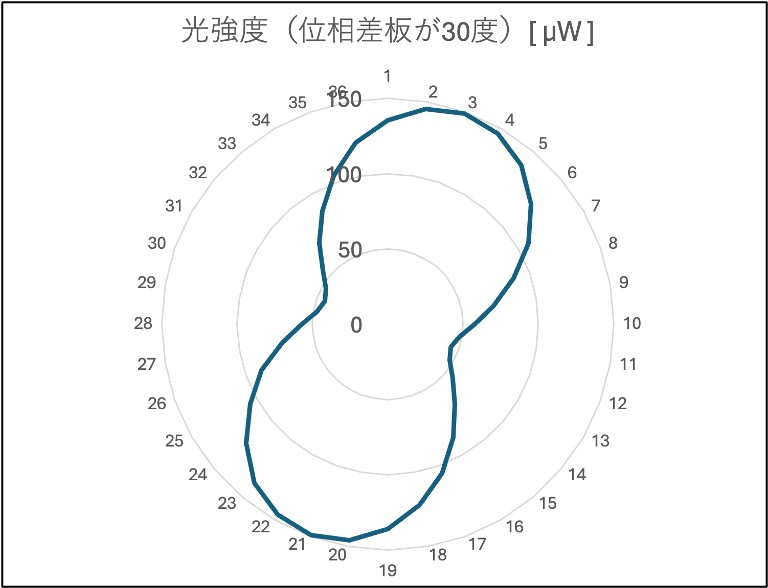
\includegraphics{/Users/kiloverse/Documents/物理学実験2/光の偏光/report_fig/実験Bレーザー30.jpg}}
          \caption{実験B:角度ごとの光強度レーザー図(30°)}
          \label{fig:19}
        \end{minipage}
    \end{figure}
    \begin{figure}[htbp]
        \centering
        \begin{minipage}[b]{0.5\textwidth} % minipage 环境用于在同一行内并排放置内容,[b] 参数表示底部对齐,{0.5\textwidth} 设置 minipage 的宽度为页面宽度的一半
          \centering
          \adjustbox{height=0.205\textheight,keepaspectratio}{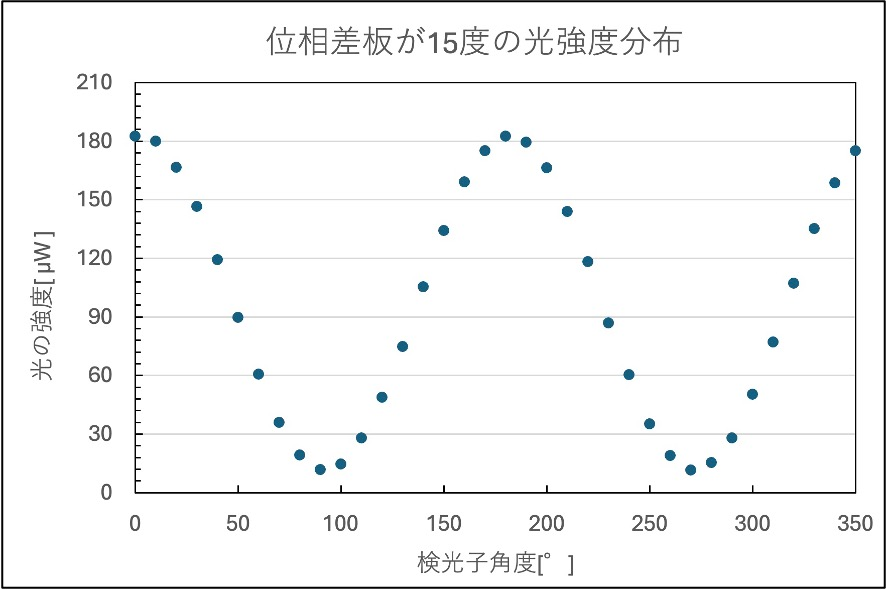
\includegraphics{/Users/kiloverse/Documents/物理学実験2/光の偏光/report_fig/実験B光強度15.jpg}} % 使用 \adjustbox 命令将图片高度设置为 0.3\textheight,根据需要调整 height 参数,以确保图片的高度合适
          \caption{実験B:光強度と検光子角度の関係(15°)}
          \label{fig:20}
        \end{minipage}% % 在两个 minipage 环境之间使用 % 符号来消除之间的空白
        \begin{minipage}[b]{0.5\textwidth}
          \centering
          \adjustbox{height=0.205\textheight,keepaspectratio}{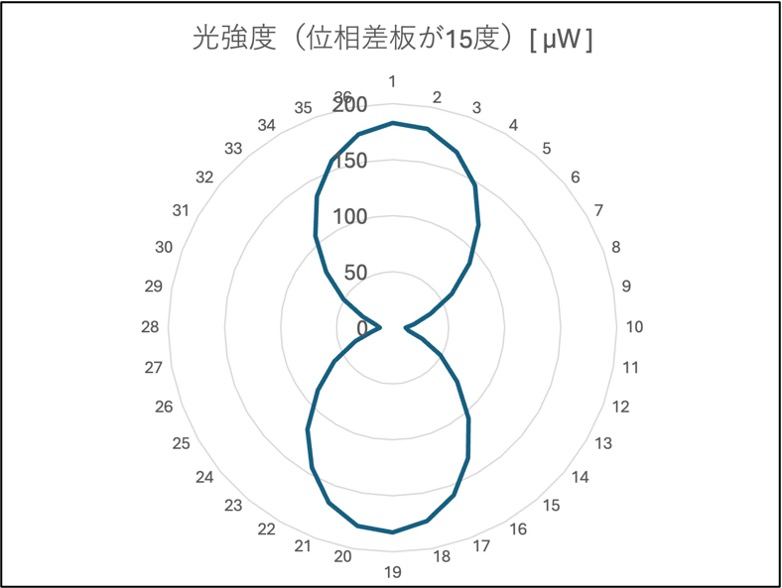
\includegraphics{/Users/kiloverse/Documents/物理学実験2/光の偏光/report_fig/実験Bレーザー15.jpg}}
          \caption{実験B:角度ごとの光強度レーザー図(15°)}
          \label{fig:21}
        \end{minipage}
    \end{figure}
    \begin{figure}[htbp]
        \centering
        \begin{minipage}[b]{0.5\textwidth} % minipage 环境用于在同一行内并排放置内容,[b] 参数表示底部对齐,{0.5\textwidth} 设置 minipage 的宽度为页面宽度的一半
          \centering
          \adjustbox{height=0.205\textheight,keepaspectratio}{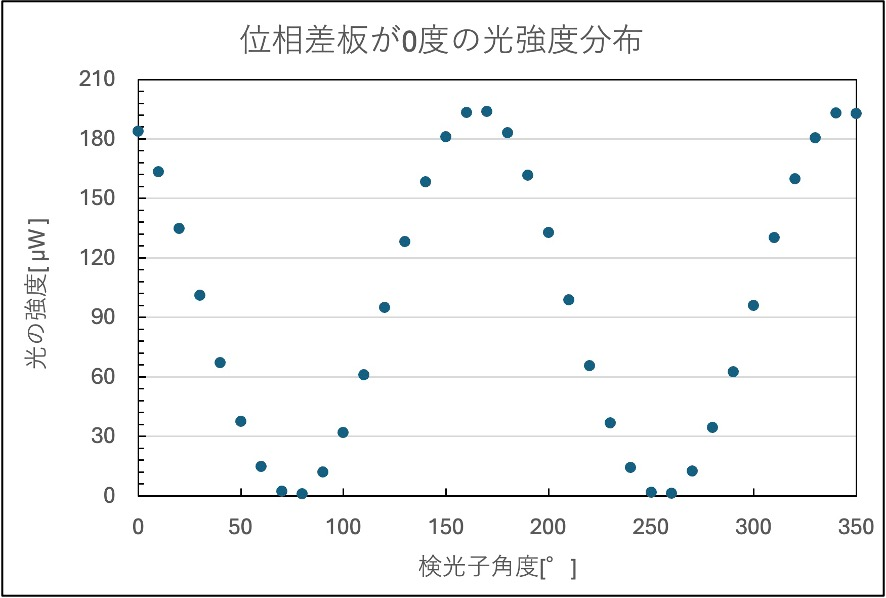
\includegraphics{/Users/kiloverse/Documents/物理学実験2/光の偏光/report_fig/実験B光強度0.jpg}} % 使用 \adjustbox 命令将图片高度设置为 0.3\textheight,根据需要调整 height 参数,以确保图片的高度合适
          \caption{実験B:光強度と検光子角度の関係(0°)}
          \label{fig:22}
        \end{minipage}% % 在两个 minipage 环境之间使用 % 符号来消除之间的空白
        \begin{minipage}[b]{0.5\textwidth}
          \centering
          \adjustbox{height=0.205\textheight,keepaspectratio}{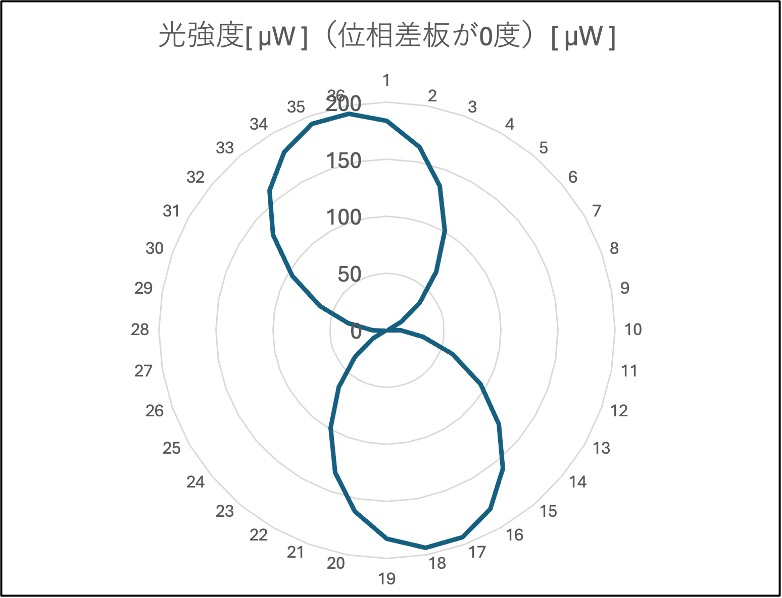
\includegraphics{/Users/kiloverse/Documents/物理学実験2/光の偏光/report_fig/実験Bレーザー0.jpg}}
          \caption{実験B:角度ごとの光強度レーザー図(0°)}
          \label{fig:23}
        \end{minipage}
    \end{figure}
    \FloatBarrier
\end{spacing}

\subsubsection*{結果の解析}
\begin{spacing}{1.2}
    \begin{enumerate}[label=\arabic*), before=\begin{spacing}{1.2}, after=\end{spacing}] % \arabic阿拉伯数字,\roman小写罗马数字,\Roman,\alph小写字母,\Alph,“*”之后添加自己喜欢的序号后样式, 如1.添加“.”,1)添加“)”;利用{spacing}自定义\item内的行间距
    \item 
    実験3と実験Bの結果から、
    楕円偏光の生成が理論と一致していることが確認された。
    実験3のレーザー図に描かれたきれいな楕円の図形(図17)は、
    位相差板を通過する光の偏光特性がうまく制御されていることを示している。
    位相差板が光の波長に応じて特定の位相シフトを引き起こすため、
    検光子を回転させると、光の強度が周期的に変化し、楕円偏光が形成された。
    これは、光の電場ベクトルが位相差板により二つの互いに直交する成分に分割され、
    それぞれが異なる位相変化を経て再合成されるためである。

    \item 
    実験3では位相差板が固定され、検光子が回転する中で、
    位相差板の角度が0度、15度、30度、45度に設定された際に観測される楕円偏光が、
    実験2の結果と対応しており、
    光強度が最大となるのは位相差板が0度のときであり、45度で最小になることが示された。
    
    \item 
    実験Bでは異なる位相差板の角度での光強度の変化が測定され、
    楕円偏光の形状が角度に応じて変化する様子が観察された。
    具体的に、図19 $\cdot$図21 $\cdot$図23のレーザー図における
    図形の対称軸は15°ずつ回転しており、
    位相差板の角度が楕円偏光の形成した図形に直接的な影響を与えることを示した。
    \end{enumerate}
\end{spacing}

\subsubsection{考察}
\subsubsection*{楕円率と位相差}
\begin{spacing}{1.2}
    実験3の図17の楕円の楕円率より、
    位相差を求めることができる[1]。
    楕円のs軸(x軸)及びf軸(y軸)方向に、
    位相差$\Delta$の電場ベクトルを射影し、
    \begin{align*}
        x &\equiv \frac{E_x}{E_0} = \cos \omega t, \\
        y &\equiv \frac{E_y}{E_0} = \cos(\omega t + \Delta).
    \end{align*}
    とし、 $t$ を消去すると、
    \begin{align*}
        y &= \cos \omega t \cos \Delta - \sin \omega t \sin \Delta \\
        y &= x \cos \Delta - \sqrt{1 - x^2} \sin \Delta \\
    \end{align*}
    となる。楕円の式まで整理すると、
    \begin{align*}
        x \cos \Delta - y &= \sqrt{1 - x^2} \sin \Delta \\
        x^2 \cos^2 \Delta + y^2 - 2xy \cos \Delta &= \sin^2 \Delta - x^2 \sin^2 \Delta \\
        x^2 + y^2 - 2xy \cos \Delta &= \sin^2 \Delta
    \end{align*}
    この式をさらに楕円の標準形 $x^2/a^2 + y^2/b^2 = 1$ に変形する。
    \begin{align*}
    \frac{x^2}{a^2} + \frac{y^2}{b^2} = \dfrac{x^2}{\dfrac{\sin^2\Delta}{1 - \cos\Delta}} + \dfrac{y^2}{\dfrac{\sin^2\Delta}{1 + \cos\Delta}} = 1,
    \end{align*}
    ここで、
    $b^2 (1 + \cos\Delta) = a^2 (1 - \cos\Delta)$ 
    の関係を確認し、
    これが楕円の性質とどのように関連しているかを説明できる。
    $\gamma \equiv b^2/a^2$ とおくと、
    \begin{align}
        \gamma (1 + \cos\Delta) = 1 - \cos\Delta \notag \\
        \Delta = \arccos \dfrac{1 - \gamma}{1 + \gamma}
    \end{align}

    実験3において、光強度の最大値が112.5 $\mu W$で、
    最小値が83.8 $\mu W$である。
    よって、楕円の短軸と長軸の比 
    $b^2 / a^2 = (83.8 / 112.5)^2$ が得られる。
    式(7)に代入して、
    \begin{align*}
        \Delta = 1.280 \approx 0.41 \pi
    \end{align*}
    という位相差が求められた。
    $\Delta = 0.41 \pi \not= n\pi/2$であることは
    楕円偏光が生じることを示唆している。
    実験3と実験Bで観察できた楕円偏光と一致しており、
    実験によって、楕円偏光の形状や特性についての理論を確認でき、
    理解を深めることができた。
\end{spacing}

\subsubsection*{他の実験との比較}
\begin{spacing}{1.2}
    自分の実験結果の妥当性を確認するために、
    他のグループからデータを拝借した。
    他のグループの実験3の楕円偏光は図24の通りである。\\
    \begin{wrapfigure}{r}{0.3\textwidth} % 开始一个环绕图片的环境, {r}:图片靠右(l 表示图片靠左), {0.4\textwidth}:设置图片区域占据的宽度为页面宽度的 40%
        \fbox{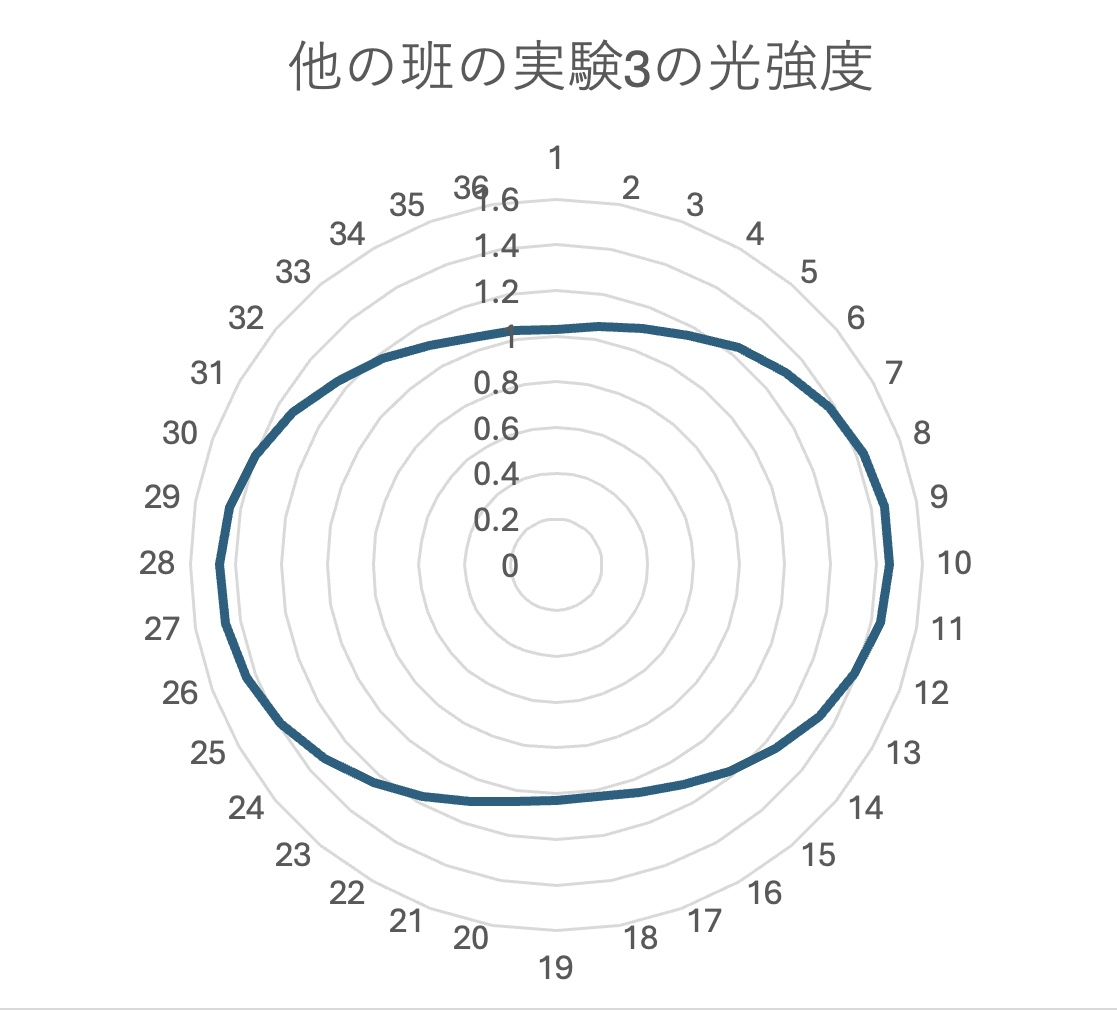
\includegraphics[width=0.26\textwidth]{/Users/kiloverse/Documents/物理学実験2/光の偏光/report_fig/工藤実験3.JPG}}
        \caption{他のグループの実験3の結果}
        \label{fig:24}
    \end{wrapfigure}
    \indent
    ここで、光強度の最大値が147 $\mu W$で、
    最小値が103 $\mu W$である。
    よって、楕円の短軸と長軸の比 
    $b^2 / a^2 = (103 / 147)^2$ が得られる。
    式(7)に代入して、位相差が
    \begin{align*}
        \Delta = 1.22 \approx 0.39 \pi
    \end{align*}
    となった。自分の実験で推測された位相差$\Delta = 0.41\pi$と比較して、
    $0.02 \pi$の誤差は、実験装置の設定や実験環境の違い、
    さらには測定精度の差異に起因すると考えられる。

    光検出器のセットアップにおける微妙な違いは、
    実験結果に大きな影響を与える可能性がある。
    光検出器の位置や角度のわずかなずれも、
    測定される光強度に影響を及ぼす。
    また、本実験では、光強度の精度が0.1 $\mu W$に達しているが、
    他のグループでは精度が1 $\mu W$までであり、
    この精度の違いが位相差の推測値に誤差を生じさせる原因となっている可能性が高い。

    以上の分析から、
    自分の実験結果の妥当性が確認でき、
    信頼性があると評価できる。
    ただし、さらなる精度向上のためには、
    光検出器のセットアップの最適化や実験環境のさらなる制御が必要である。
\end{spacing}

\subsubsection*{楕円偏光の軸}
\begin{spacing}{1.2}
    実験3と実験Bから得られた光強度分布を比較してみると、
    図25通りの位相差板角度ごとの光強度分布の遷移図が得られた。
    この遷移図から、楕円偏光の軸が位相差板の角度に応じて変化する様子が観察されている。
    \begin{figure}[!htb] % 选项 [htbp] 代表位置优先级, “here, top, bottom, page” 分别表示:此处、页顶、页底、单独一页
        \centering
        \fbox{\adjincludegraphics[width=0.618\textwidth, keepaspectratio]{/Users/kiloverse/Documents/物理学実験2/光の偏光/report_fig/実験3実験B遷移図.JPG}}
        \caption{実験3と実験Bの楕円偏光の比較}
        \label{fig:25}
    \end{figure}
    \FloatBarrier
    楕円偏光の軸とは、偏光された光の主要な電場ベクトルの方向を指し、
    この軸は位相差板を通過する光の波長や位相差に応じて変化する。
    位相差板の角度が異なると、楕円偏光の長軸と短軸がそれに応じて回転し、
    楕円の形状が変わる。

    図25より、位相差板の角度が0度、15度、30度、および45度の場合の
    楕円偏光の形状を示しており、
    位相差板が楕円偏光の軸および形状に直接的な影響を与えていることが確認できた。
    具体的には、位相差板が0度の場合に光強度が最大となり、
    45度の場合に最小となることが、楕円の形状からも明示された。
    これは、実験2通りに、
    位相差板を通過する光の偏光状態が位相差によって周期的に変化していることを示した。
\end{spacing}

\subsection{考察のまとめ}
\subsubsection{誤差原因の解析}
\begin{enumerate}[label=\alph*), before=\begin{spacing}{1.2}, after=\end{spacing}] % \arabic阿拉伯数字,\roman小写罗马数字,\Roman,\alph小写字母,\Alph,“*”之后添加自己喜欢的序号后样式, 如1.添加“.”,1)添加“)”;利用{spacing}自定义\item内的行间距
    \item 実験配置の不正確さは、測定データに大きな誤差をもたらす主な原因である。
    特にポラロイドの角度の設定と光検出器の固定が不適切な場合、
    光の進行方向と偏光子、位相差板、検光子の配置が理想的な位置からずれてしまうことがある。
    これにより、光の透過や反射が理論通りに行われず、測定される光強度に誤差が生じる。
    また、光検出器がしっかりと固定されていないと、実験中の動きによっても測定値に影響が出る。
    \item 光学系の各要素の品質が十分でない場合、実験結果に誤差が生じる。
    偏光子や位相差板、検光子の光学的特性が不均一であったり、
    表面に傷や汚れがあったりすると、
    光の偏光状態が均一でなくなり、予期されない光の散乱や吸収が発生する可能性がある。
    \item 実験室内の環境光や外光の影響も、光学実験における誤差の一つの成因である。
    実験中に周囲からの光が漏れ入ると、
    特に偏光や楕円偏光の測定においては、
    本来の光のパターンに追加の光が混入し、
    測定データが不正確になる可能性がある。
\end{enumerate}
\subsubsection{改善点}
\begin{enumerate}[label=\alph*), before=\begin{spacing}{1.2}, after=\end{spacing}] % \arabic阿拉伯数字,\roman小写罗马数字,\Roman,\alph小写字母,\Alph,“*”之后添加自己喜欢的序号后样式, 如1.添加“.”,1)添加“)”;利用{spacing}自定义\item内的行间距
    \item 実験装置を正確に設置するためには、
    光路が歪みなく、ポラロイドの中心を通過するようにチェックする必要がある。
    今回の実験では、光路をチェックしようとした時、
    強光で目が痛くなってしまったので、このステップを飛ばした。
    今後の実験で、目を保護するメガネを事前に準備するのがおすすめである。
    また、光検出器の固定も見直し、
    振動や外部からの衝撃に強くするように、
    テープでしっかり固定すると、測定時の誤差を減らせる。
    \item 偏光子や位相差板、検光子など
    光学部品の品質を高めるためには、
    実験する前に品質チェックが必要です。
    実験用光学系は定期的に検査を行い、
    問題があれば使わないようにする。
    また、予めポラロイドを掃除して、
    汚れやキズが光を通すことに影響しないようにすることが大切だと思う。
    \item 外部からの光の侵入を防ぐために、
    実験中には室内の照明を極力抑え、
    あるいは暗室で実験を行うことで、
    外光による干渉を最小限に抑えることができる。
    \item フィッティングの妥当性を高めるためには、
    入射光強度を実験で測定することが重要だ。
    可能であれば、光源から直接光強度を測定する装置を設置するか、
    実験前に光源の校正を行った方がいいと思う。
    これにより、フィッティングで用いるデータの精度が向上し、
    より正確な結果を得ることができる。
\end{enumerate}

\section{実験結論}
\begin{enumerate}[label=\arabic*), before=\begin{spacing}{1.2}, after=\end{spacing}] % \arabic阿拉伯数字,\roman小写罗马数字,\Roman,\alph小写字母,\Alph,“*”之后添加自己喜欢的序号后样式, 如1.添加“.”,1)添加“)”;利用{spacing}自定义\item内的行间距
    \item 実験1によって、マリュスの法則が検証され、
    光強度が検光子の角度に応じて $\cos^2 \theta$ に比例することが確認さできた。
    理論曲線と実測データの一致が顕著であり、
    偏光子と検光子の透過軸の角度による光強度の変化が法則通りであることが確認された。
    \item ポラロイドの性質を調べた。
    偏光子と検光子の透過軸のなす角度により、光の透過強度が異なることがわかった。
    特に、直交ニコル法と平行ニコル法を用いて、光の偏光状態の変化を観察し、
    ポラロイドの透過軸の位置が光強度に与える影響を調べた。
    \item 位相差板の光学的異方性について理解を深めた。
    具体的に、位相差板によって光が通過する際に生じる位相差を測定し、
    その結果を理論モデルと比較した。
    位相差板が異なる偏光成分に対して異なる屈折率を示すため、
    光の偏光状態が変化し、位相差が生じることがわかった。
    これにより、位相差板の光学的性質が光強度と偏光状態に与える影響を詳細に解析することができた。
    \item 偏光状態について調べて、
    直線偏光、円偏光、楕円偏光の各偏光状態の特性を理解し、
    特に楕円偏光の性質と楕円偏光の軸について詳しく調査した。
    実験3と実験Bの結果から、楕円偏光の形状が位相差板の角度に応じて変化することが確認された。
    楕円偏光の軸が位相差板の角度により変化する様子を観察し、
    楕円偏光の生成メカニズムとその特性を理解することができた。
\end{enumerate}


% 参考文献 %%%%%%%%%%%%%%%%%%%%%%%%%%%%%%%%%%%%%%%%%%%%%%%%%%
\section*{参考文献}
\begin{spacing}{1.4}
    \noindent
    [1] 6.偏光. 
    東京理科大学, 
    \url{https://letus.ed.tus.ac.jp/pluginfile.php/2417711/mod_resource/content/9/%E5%81%8F%E5%85%89%E3%81%AE%E3%83%86%E3%82%AD%E3%82%B9%E3%83%88.pdf}
    (参照2024-06-29)

    \noindent
    [2] 荻野研究室. 
    ポリビニルアルコールについて③-偏光フィルムを使った実験②-, 
    \url{https://web.tuat.ac.jp/~oginolab/japanese/essay/20190818/20190818.html}
    (参照2024-06-29)

    \noindent
    [3] 実験手順改訂版. 
    東京理科大学, 
    \url{https://letus.ed.tus.ac.jp/pluginfile.php/2172159/mod_resource/content/7/%E5%AE%9F%E9%A8%93%E6%89%8B%E9%A0%86_%E6%94%B9%E8%A8%82%E7%89%88.PDF}
    (参照2024-06-30)

    \noindent
    [4] セロハンテープと偏光板を用いた円偏光子の作製と性能評価. 
    千葉大学, 
    \url{https://opac.ll.chiba-u.jp/da/curator/107994/S24326291-4-P157.pdf}
    (参照2024-07-01)

    \noindent
    [5] 波長板(1/2,1/4…etc)の用途や動作原理とは. 
    テクノロジー, 
    \url{https://www.fiberlabs.co.jp/tech-explan/about-wave-plate/}
    (参照2024-06-21)

    \noindent
    [6] 複屈折に関して. AUTODESK, 
    \url{https://help.autodesk.com/view/MFC/2024/JPN/?guid=MoldflowComm_CLC_Analyses_analysis_sequences_Birefringence_analysis_About_Birefringence_html}
    (参照2024-06-22)

    \noindent
    [7] KOBRA技術資料.
    \url{https://oji-keisoku.co.jp/cms/uploads/kobra_tech.pdf}
    (参照2024-06-22)

    \noindent
    [8] 偏光顕微鏡法(Polarized Optical Microscopy). 公益社団法人高分子学会, 
    \url{https://www.spsj.or.jp/equipment/news/news_detail_75.html}
    (参照2024-06-23)
\end{spacing}

\newpage
\section*{付録}
\subsection*{実験Aで使用されたフィッティングコード}
\begin{lstlisting}
import numpy as np
import matplotlib.pyplot as plt
from scipy.optimize import curve_fit

# 実測データ
theta_deg = np.array([0, 10, 20, 30, 40, 50, 60, 70, 80, 90, 100, 110, 120, 130, 140, 150, 160, 170, 180, 190, 200, 210, 220, 230, 240, 250, 260, 270, 280, 290, 300, 310, 320, 330, 340, 350])
intensity = np.array([158.7, 119.8, 91.6, 86, 106.5, 143.4, 178.3, 196.7, 188.6, 157.1, 119.4, 90.7, 85.8, 107.3, 143.8, 179.6, 197.5, 189.3, 158.5, 120.1, 90.9, 86.2, 106.5, 144, 179.7, 197.4, 189.5, 158.7, 119.9, 90.5, 85.3, 106.1, 143.8, 178, 196.2, 187.5])

# 角度を rad に変換
theta_rad = np.deg2rad(theta_deg)

# 平行ニコルの理論式
def intensity_model(theta, I_0, alpha, delta):
    theta = theta + alpha # 位相差板の光軸の位置をfitするために alpha を加算
    return I_0 * (1 - np.sin(2 * theta)**2 * np.cos(delta / 2)**2)

# fitting
popt, pcov = curve_fit(intensity_model, theta_rad, intensity, p0 = [239.1, 0, np.pi/2]) # 実験1で測定した光強度の最大値を光源強度の初期値とする
I_0_fit, alpha_fit, delta_fit = popt

# fitting の結果を output
print("I_0 = ", I_0_fit)
print("alpha_rad = ", alpha_fit)
print("alpha_deg = ", np.rad2deg(alpha_fit))
print("delta_rad = ", delta_fit)
print("delta_deg = ", np.rad2deg(delta_fit))

# フィッティング結果を用いて理論値を計算
theta_fit = np.linspace(0, 2 * np.pi, 500)
intensity_fit = intensity_model(theta_fit, I_0_fit, alpha_fit, delta_fit)

# プロット
plt.figure(figsize=(10, 6))
plt.plot(np.rad2deg(theta_fit), intensity_fit, label='theoretical intensity')  # 理论曲线
plt.scatter(theta_deg, intensity, color='red', label='experimental intensity')  # 实验数据点
plt.xlabel('theta [degree]')
plt.ylabel('Intensity [ $\mu W$]')
plt.title('Fitted Theoretical I vs Experimental I (open nicol)')
plt.legend()
plt.grid(True)
plt.ylim(0, 250) # Excel 図と統一するように y 軸の範囲を set
plt.show()
\end{lstlisting}

\subsection*{実験2のフィッティングに通過率rを導入する}
\begin{lstlisting}
import numpy as np
import matplotlib.pyplot as plt
from scipy.optimize import curve_fit

# 実測データ
theta_deg = np.array([0, 10, 20, 30, 40, 50, 60, 70, 80, 90, 100, 110, 120, 130, 140, 150, 160, 170, 180, 190, 200, 210, 220, 230, 240, 250, 260, 270, 280, 290, 300, 310, 320, 330, 340, 350])
intensity = np.array([37.8, 77.6, 106.7, 112.5, 92, 55.5, 19.6, 0.8, 8.1, 38.4, 77.4, 106.5, 112.2, 92.2, 55.1, 19.8, 0.7, 8.3, 37.4, 77, 106.9, 112.5, 92.2, 55.9, 19.5, 0.7, 7.3, 37.8, 77.8, 106.6, 113, 93.1, 57.2, 19.2, 0.7, 8.1])

# 角度を rad に変換
theta_rad = np.deg2rad(theta_deg)

# 直交ニコルの理論式(光透過率を含む)
def theoretical_intensity(theta, I_0, alpha, delta, r):
    theta = theta + alpha  # 位相差板の光軸の位置をfitするために alpha を加算
    return r * I_0 * np.sin(2 * theta)**2 * np.sin(delta / 2)**2

# フィッティング
popt, pcov = curve_fit(theoretical_intensity, theta_rad, intensity, p0 = [250, 0, np.pi/2, 1] , bounds=([0, -np.pi, 0, 0], [np.inf, np.pi, np.pi, 1]))
I_0_fit, alpha_fit, delta_fit, r_fit = popt

# 結果の出力
print("I_0 = ", I_0_fit)
print("alpha_rad = ", alpha_fit)
print("alpha_deg = ", np.rad2deg(alpha_fit))
print("delta_rad = ", delta_fit)
print("delta_deg = ", np.rad2deg(delta_fit))
print("r = ", r_fit)

# フィッティング結果を用いて理論値を計算
theta_fit = np.linspace(0, 2 * np.pi, 500)
intensity_fit = theoretical_intensity(theta_fit, I_0_fit, alpha_fit, delta_fit, r_fit)

# プロット
plt.figure(figsize=(10, 6))
plt.plot(np.rad2deg(theta_fit), intensity_fit, label='Theoretical Intensity')
plt.scatter(theta_deg, intensity, color='red', label='Experimental Intensity')
plt.xlabel('Theta (degrees)')
plt.ylabel('Intensity (μW)')
plt.title('Fitted Theoretical I vs Experimental I (Close Nicol)')
plt.legend()
plt.grid(True)
plt.show()
\end{lstlisting}

\newpage
\subsection*{実験Bのフィッティングに通過率rを導入する}
\begin{lstlisting}
import numpy as np
import matplotlib.pyplot as plt
from scipy.optimize import curve_fit

# 実測データ
theta_deg = np.array([0, 10, 20, 30, 40, 50, 60, 70, 80, 90, 100, 110, 120, 130, 140, 150, 160, 170, 180, 190, 200, 210, 220, 230, 240, 250, 260, 270, 280, 290, 300, 310, 320, 330, 340, 350])
intensity = np.array([158.7, 119.8, 91.6, 86, 106.5, 143.4, 178.3, 196.7, 188.6, 157.1, 119.4, 90.7, 85.8, 107.3, 143.8, 179.6, 197.5, 189.3, 158.5, 120.1, 90.9, 86.2, 106.5, 144, 179.7, 197.4, 189.5, 158.7, 119.9, 90.5, 85.3, 106.1, 143.8, 178, 196.2, 187.5])

# 角度を rad に変換
theta_rad = np.deg2rad(theta_deg)

# 平行ニコルの理論式(光の透過率を含む)
def intensity_model(theta, I_0, alpha, delta, r):
    theta = theta + alpha  # 位相差板の光軸の位置をfitするために alpha を加算
    return r * I_0 * (1 - np.sin(2 * theta)**2 * np.cos(delta / 2)**2)

# フィッティング
popt, pcov = curve_fit(intensity_model, theta_rad, intensity, p0 = [250, 0, np.pi/2, 1], bounds=([0, -np.pi, 0, 0], [np.inf, np.pi, np.pi, 1]))
I_0_fit, alpha_fit, delta_fit, r_fit = popt

# 結果の出力
print("I_0 = ", I_0_fit)
print("alpha_rad = ", alpha_fit)
print("alpha_deg = ", np.rad2deg(alpha_fit))
print("delta_rad = ", delta_fit)
print("delta_deg = ", np.rad2deg(delta_fit))
print("r = ", r_fit)

# フィッティング結果を用いて理論値を計算
theta_fit = np.linspace(0, 2 * np.pi, 500)
intensity_fit = intensity_model(theta_fit, I_0_fit, alpha_fit, delta_fit, r_fit)

# プロット
plt.figure(figsize=(10, 6))
plt.plot(np.rad2deg(theta_fit), intensity_fit, label='Theoretical Intensity')
plt.scatter(theta_deg, intensity, color='red', label='Experimental Intensity')
plt.xlabel('Theta (degrees)')
plt.ylabel('Intensity (μW)')
plt.title('Fitted Theoretical I vs Experimental I (Open Nicol)')
plt.legend()
plt.grid(True)
plt.ylim(0, 250)  # Excel 図と統一するように y 軸の範囲を set
plt.show()
\end{lstlisting}

\end{document}